\chapter{مبانی نظری توزیع کلید کوانتومی}
%=====================================================================

\section{اصول فیزیکی زیربنایی}

امنیت \lr{QKD} بر خلاف رمزنگاری کلاسیک، متکی به دشواری محاسباتی یک مسئلهٔ ریاضی نیست، بلکه مستقیماً از قوانین بنیادین مکانیک کوانتومی نتیجه می‌شود. دو اصل کلیدی در این میان نقش تعیین‌کننده دارند:

\begin{definition}[اصل عدم‌قطعیت در اندازه‌گیری]
اندازه‌گیری یک حالت کوانتومی ناشناخته در یک پایهٔ اندازه‌گیری دلخواه، به‌طور کلی آن حالت را برهم می‌زند؛ مگر آنکه پایهٔ اندازه‌گیری با پایه‌ای که حالت در آن تهیه شده، منطبق باشد.
\end{definition}

\begin{theorem}[قضیهٔ عدم-شبیه‌سازی \lr{\cite{wootters1982}}]
هیچ عملگر یکانی (فیزیکی) وجود ندارد که بتواند یک حالت کوانتومی دلخواه و ناشناخته $\lvert\psi\rangle$ را بدون تغییر در حالت اصلی، به‌طور کامل روی یک سامانهٔ کمکی کپی کند.
\end{theorem}

نتیجهٔ مستقیم این قضیه برای امنیت ارتباطات آن است که یک شنودگر \lr{(Eve)} \textbf{اصولاً نمی‌تواند} فوتون‌های حامل کلید را رهگیری، کپی و بدون تغییر ارسال کند؛ هرگونه تلاش برای اندازه‌گیری یا کپی‌برداری از حالت کوانتومی، اختلال آماری قابل‌کشفی در نرخ خطای بیت کوانتومی (تعریف در بخش \lr{2.3}) ایجاد می‌کند. این ویژگی -- که در رمزنگاری کلاسیک هیچ مابه‌ازایی ندارد -- پایهٔ \textbf{امنیت اثبات‌پذیر اطلاعاتی} \lr{(Information-Theoretic Security)} در \lr{QKD} است.

\section{پروتکل \lr{BB84}}

نخستین و پرکاربردترین پروتکل \lr{QKD}، پروتکل \lr{BB84}\LTRfootnote{Named after its inventors, Bennett and Brassard, and the publication year 1984.} است که در سال $1984$ توسط بنت و براسارد\LTRfootnote{Charles H. Bennett and Gilles Brassard} \lr{\cite{bennett1984}} پیشنهاد شد. شکل \ref{fig:bb84} گردش کار کلی این پروتکل را نشان می‌دهد.

\begin{figure}[htbp]
\centering
\begin{tikzpicture}[
  node distance=1.2cm,
  box/.style={rectangle,draw,thick,rounded corners,minimum width=2.6cm,minimum height=1cm,align=center,fill=blue!8},
]
\node[box] (alice) {\lr{Alice}\\(فرستنده)};
\node[box,right=6.3cm of alice] (bob) {\lr{Bob}\\(گیرنده)};
\draw[-{Stealth[length=3mm]},thick,blue!60!black] (alice) -- node[above,font=\footnotesize]{\rl{کانال کوانتومی (فوتون‌های تکی)}} (bob);
\draw[-{Stealth[length=3mm]},thick,red!60!black] ($(alice.south)+(0,-0.4)$) -- node[below,font=\footnotesize]{کانال کلاسیک (تطبیق پایه، تصحیح خطا، تقطیر محرمانگی)} ($(bob.south)+(0,-0.4)$);
\node[below=1.1cm of alice, align=right, font=\footnotesize] (a2) {\lr{1.} تولید بیت‌های تصادفی\\\lr{2.} انتخاب تصادفی پایه ($+/\times$)\\\lr{3.} کدگذاری و ارسال قوبیت‌ها};
\node[below=1.1cm of bob, align=right, font=\footnotesize] (b2) {\lr{1.} انتخاب تصادفی پایهٔ اندازه‌گیری\\\lr{2.} اندازه‌گیری قوبیت‌ها\\\lr{3.} غربال‌سازی کلید \lr{(Key Sifting)}};
\end{tikzpicture}
\caption{شمای کلی پروتکل \lr{BB84}: تبادل کلید کوانتومی بین \lr{Alice} و \lr{Bob}}
\label{fig:bb84}
\end{figure}

برای نمایش دقیق‌تر ترتیب زمانی پیام‌ها میان دو طرف، شکل \ref{fig:bb84seq} همان پروتکل را در قالب نمودار توالی \lr{(Sequence Diagram)} نشان می‌دهد که هفت گام اصلی توضیح داده‌شده در ادامه را به‌ترتیب دربر می‌گیرد.

\begin{figure}[htbp]
\centering
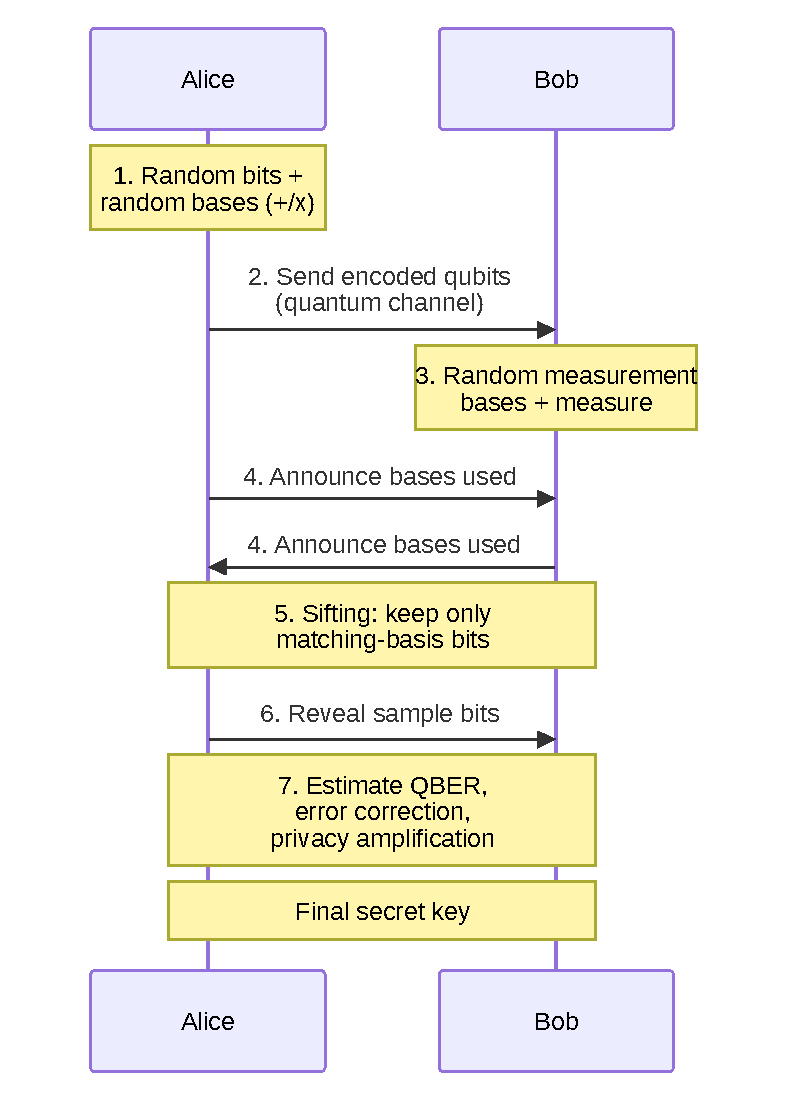
\includegraphics[width=0.75\linewidth]{figs/fig_bb84_sequence.pdf}
\caption{نمودار توالی زمانی پروتکل \lr{BB84} از تولید بیت تصادفی تا استخراج کلید نهایی}
\label{fig:bb84seq}
\end{figure}

مراحل اصلی پروتکل \lr{BB84} به شرح زیر است:

\begin{enumerate}
\item \textbf{تهیهٔ حالت \lr{(State Preparation)}:} \lr{Alice} برای هر بیت کلید، به‌صورت تصادفی یکی از دو پایهٔ متعامد -- پایهٔ مستطیلی ($+$) یا پایهٔ قطری ($\times$) -- را انتخاب کرده و بیت را روی حالت قطبش فوتون کدگذاری می‌کند.
\item \textbf{انتقال:} فوتون‌ها از طریق کانال کوانتومی (معمولاً فیبر نوری تاریک \lr{(Dark Fiber)} در طول‌موج $1550$ نانومتر یا کانال فضای آزاد/ماهواره‌ای) به \lr{Bob} ارسال می‌شوند.
\item \textbf{اندازه‌گیری:} \lr{Bob} برای هر فوتون دریافتی، به‌طور مستقل و تصادفی یکی از دو پایه را برای اندازه‌گیری انتخاب می‌کند.
\item \textbf{تطبیق پایه \lr{(Basis Reconciliation)}:} \lr{Alice} و \lr{Bob} از طریق یک کانال کلاسیک \textbf{احراز‌هویت‌شده} (نه لزوماً محرمانه)، پایه‌های انتخابی خود را -- بدون افشای مقدار بیت‌ها -- مقایسه کرده و تنها بیت‌هایی را نگه می‌دارند که در آن‌ها پایهٔ فرستنده و گیرنده یکسان بوده است. این مرحله «کلید غربال‌شده» \lr{(Sifted Key)} را تولید می‌کند.
\item \textbf{برآورد نرخ خطا و تصحیح خطا:} با مقایسهٔ زیرمجموعه‌ای تصادفی از کلید غربال‌شده، نرخ خطای بیت کوانتومی برآورد می‌شود.
\item \textbf{تقطیر محرمانگی \lr{(Privacy Amplification)}:} با استفاده از توابع درهم‌سازی جهانی \lr{(Universal Hashing)}، طول کلید کاهش داده می‌شود تا هرگونه اطلاعات نشت‌یافته به شنودگر عملاً به صفر برسد و «کلید نهایی امن» تولید شود.
\end{enumerate}

\section{نرخ خطای بیت کوانتومی و نرخ کلید امن}

نرخ خطای بیت کوانتومی \lr{(Quantum Bit Error Rate -- QBER)} مهم‌ترین شاخص کیفیت و امنیت یک پیوند \lr{QKD} است و به‌صورت زیر تعریف می‌شود:

\begin{equation}
\label{eq:qber}
\mathrm{QBER} = \frac{N_{\text{error}}}{N_{\text{total}}}
\end{equation}

که در آن $N_{\text{error}}$ تعداد بیت‌های نادرست در نمونهٔ آزمایش‌شده و $N_{\text{total}}$ تعداد کل بیت‌های غربال‌شدهٔ نمونه‌برداری‌شده است. در عمل، یک آستانهٔ امنیتی مشخص (برای \lr{BB84} معمولاً در حدود $11\%$) وجود دارد که فراتر از آن، امکان استخراج کلید امن از نظر تئوری اطلاعات وجود ندارد و ارتباط باید قطع شود.

با در نظر گرفتن اثرات عملی نظیر تلفات کانال، نویز آشکارساز و حملات نشت‌اطلاعات از کانال جانبی، نرخ کلید امن نهایی $R$ با فرمول تعمیم‌یافتهٔ \lr{GLLP}\LTRfootnote{Gottesman, Lo, Lütkenhaus, and Preskill} \lr{\cite{gllp2004}} به‌صورت زیر تخمین زده می‌شود:

\begin{align}
\label{eq:gllp}
R \;\geq\; q \Big\{ -Q_{\mu}\, f(E_{\mu})\, H_2(E_{\mu}) \;+\; Q_1 \big[1 - H_2(e_1)\big] \Big\}
\end{align}

که در آن $q$ کارایی پروتکل (برای \lr{BB84} با غربال‌سازی معمولی $q=1/2$)، $Q_{\mu}$ نرخ شمارش کلی، $E_{\mu}$ نرخ خطای کلی، $f(E_{\mu})$ کارایی الگوریتم تصحیح خطا (معمولاً بین $1.1$ تا $1.2$)، $Q_1$ و $e_1$ به‌ترتیب نرخ شمارش و نرخ خطای رویدادهای تک‌فوتونی، و $H_2(\cdot)$ تابع آنتروپی دودویی شانون است:

\begin{equation}
H_2(x) = -x\log_2(x) - (1-x)\log_2(1-x)
\end{equation}

این رابطه نشان می‌دهد که نرخ کلید امن با افزایش فاصلهٔ انتقال (و درنتیجه افزایش تلفات و کاهش $Q_1$) به‌صورت نمایی افت می‌کند -- محدودیتی بنیادین که در فصل بعد، معماری‌های عملی برای غلبه بر آن معرفی می‌شوند.

%=====================================================================
